%\documentclass[notes]{beamer}
\documentclass[]{beamer}
% Class options include: notes, notesonly, handout, trans,
%                        hidesubsections, shadesubsections,
%                        inrow, blue, red, grey, brown

\usepackage{graphicx}
\usepackage{booktabs}
\usepackage{tikz}
\usepackage{url}

\usetheme{Madrid}
\usecolortheme{dolphin}
%\usecolortheme{seagull}
%\usecolortheme{seahorse}
\useoutertheme{infolines}
\useinnertheme{rectangles}
%\useoutertheme[footline=authortitle]{miniframes}

\setbeamercolor{block title}{bg=blue}
%\setbeamerfont*{title}{size=\huge}

\setbeamerfont{itemize/enumerate body}{size=\LARGE}
\setbeamerfont{itemize/enumerate subbody}{size=\Large}
\setbeamerfont{itemize/enumerate subsubbody}{size=\footnotesize}

\DeclareMathOperator*{\argmax}{arg\,max}

% Theme for beamer presentation.
%\usepackage{beamerthemesplit} 
%\usepackage{beamerthemelined} 
% Other themes include: beamerthemebars, beamerthemelined, 
%                       beamerthemetree, beamerthemetreebars  

\beamertemplatenavigationsymbolsempty

\makeatletter
\setbeamertemplate{footline}
{
  \leavevmode%
  \hbox{%
  \begin{beamercolorbox}[wd=\paperwidth,ht=2.25ex,dp=1ex,right]{date in head/foot}%
    \usebeamerfont{date in head/foot}\insertshortdate{}\hspace*{2em}
    \insertframenumber{} / \inserttotalframenumber\hspace*{2ex} 
  \end{beamercolorbox}}%
  \vskip0pt%
}
\makeatother

%\setbeamercolor*{title}{bg=gray,fg=blue}
\title{Naive Bayes Spam Filtering\\Using Word-Position-Based Attributes}    % Enter your title between curly braces
\author{Johan Hovold}                 % Enter your name between curly braces
\institute{Dejun Qian}      % Enter your institute name between curly braces
%\date{\today}                    % Enter the date or \today between curly braces
\date{}                    % Enter the date or \today between curly braces

\begin{document}

% Creates title page of slide show using above information
\begin{frame}
  \titlepage
\end{frame}
\note{
\fontsize{14}{12}\selectfont
Good afternoon, everyone. My name is Dejun Qian. Today I will talk about the paper "Naive Bayes Spam Filtering Using Word-Position-Based Attributes". It is written by Johan, and published in 2004.
}

\section{Introduction}
\begin{frame}[t]{\centerline{Outline}}
  \tableofcontents
\end{frame}
\note{}

\begin{frame}[t]{\centerline{Introduction}}
  \ \\
  \begin{itemize}
  \item The problem of spam gets worse every year
  \begin{itemize}
  \item Waste resources on the Internet
  \item Waste time for user
  \item May expose children to unsuitable contents (e.g. pronography)
  \end{itemize}
  \ \\
  \ \\
\pause
  \item The solution to the spam problem
  \begin{itemize}
  \item Automatic spam filter
  \end{itemize}
  \end{itemize}
\end{frame}
\note{}

%\begin{frame}[t]{\centerline{Difference from Text Categorisation}}
%  \ \\
%  \fontsize{14}{12}\selectfont
%  \begin{itemize}
%  \item Greater class heterogeneity
%  \begin{itemize}
%  \item Not the contents that define spam, but the fact that it is unsolicited
%  \item Legitimate messages may also span a number of diverse subjects
%  \end{itemize}
%  \ \\
%  \ \\
%  \item Difference between classes
%  \begin{itemize}
%  \item Misclassifying a legitimate message is generally much worse than misclassifying a spam
%  \end{itemize}
%  \end{itemize}
%\end{frame}
%\note{}

%\subsection{Problems}
\begin{frame}[t]{\centerline{Techniques for Spam Filters}}
  \ \\
  \fontsize{14}{12}\selectfont
  \begin{itemize}
  \item Instances of knowledge engineering
  \begin{itemize}
  \item Hand-crafted rules (e.g. presence of string ``buy now" indicates spam)
%  \item Requires both knowledge and time
%  \item Rules were supplied by the developers of the filter
%  \item Having common and, more or less, publicly available rules made it easy for spammers to construct their e-mails to get through the filter
  \end{itemize}
  \ \\
  \ \\
\pause
  \item Machine learning
  \begin{itemize}
  \item Supervised learning algorithm is presented with a mailbox and outputs a filter
%  \item E-mails have previously been classified manually as spam or non-spam
%  \item Advantage of being optimised for the e-mail distribution of the individual user
%  \item Able to use also the characteristics of non-spam, or legitimate, e-mails
  \end{itemize}
  \ \\
  \ \\
\pause
  \item Naive Bayes classifier in this paper
  \end{itemize}
\end{frame}
\note{}

\section{Naive Bayes Using Word-Position-Based Attributes}
%\begin{frame}[t]{\centerline{Outline}}
%  \tableofcontents[currentsection]
%\end{frame}
%\note{}

\begin{frame}[t]{\centerline{Naive Bayes Using Word-Position-Based Attributes}}
\ \\
  \fontsize{14}{12}\selectfont
  \begin{itemize}
  \item NB: $C_{NB}=\argmax_{c \in C} P(c) \prod_{i} P(a_i | c)$
\pause
  \item One attribute for each word position in a document
\pause
  \item Probability of certain word $w_k$ at position $i$, given target $c_j$: $P(a_i = w_k | c_j)$
\pause
  \item Sparseness: $P(a_i = w_k | c_j) = P(a_m = w_k | c_j)$
\pause
  \item Estimate $P(a_i = w_k | c_j)$ with $P(w_k | c_j)$
\pause
  \item $P(w_k | c_j) = \frac{C_j(w_k)+1}{n_j+|Vocabulary|}$
  \end{itemize}
\end{frame}
\note{}

\section{Experimental Results}
%\begin{frame}[t]{\centerline{Outline}}
%  \tableofcontents[currentsection]
%\end{frame}
%\note{}

\begin{frame}[t]{\centerline{Benchmark Corpora}}
  \begin{center}
  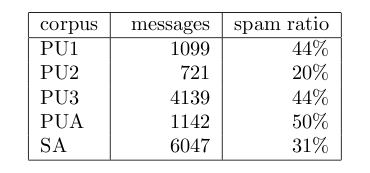
\includegraphics[width=.65\textwidth]{benchmark}
  \end{center}
  \ \\
  \fontsize{14}{12}\selectfont
  \begin{itemize}
  \item PU corpora\footnote{\texttt{\url{http://www.iit.demokritos.gr/skel/i-config/}}}
  \item SpamAssassin corpus\footnote{\texttt{\url{http://spamassassin.org/publiccorpus/}}}
  \end{itemize}
  \ \\
  \ \\
\end{frame}
\note{
\fontsize{12}{12}\selectfont
The four corpora contain private mailboxes of four different users in encrypted form. The messages have been preprocessed and stripped from attachments, HTML-tags and mail headers (except Subject). This may lead to overly pessimistic results since attachments, HTML-tags and mail headers may add useful information to the classification process.

Consists of private mail, donated by different users, in unencrypted form with headers and attachments retained. The fact that the e-mails are collected from different distributions may lead to overly optimistic results, e.g. if (some of) the spam messages have been sent to a particular address, but none of the legitimate messages have. On the other hand, the fact that the legitimate messages have been donated by different users may lead to underestimates since this should imply greater diversity of the topics of legitimate e-mails.
}

\begin{frame}[t]{\centerline{Attribute Selection - Infrequent}}
  \begin{center}
  \includegraphics[width=.7\textwidth]{infrequent}
  \end{center}
\ \\
  \begin{itemize}
  \fontsize{12}{11}\selectfont
  \item Slightly increased precision at the expense of slightly reduced recall as n grew
  \end{itemize}
\end{frame}
\note{
  \begin{itemize}
  \fontsize{12}{11}\selectfont
  \item Removing infrequent tokens had a dramatic impact on the vocabulary size
  \item Removing tokens occurring less than three times seems to be a good trade-off between memory usage and classification performance, reducing the vocabulary size with 56--69\%
  \end{itemize}
}

\begin{frame}[t]{\centerline{Attribute Selection - Frequent}}
  \begin{center}
  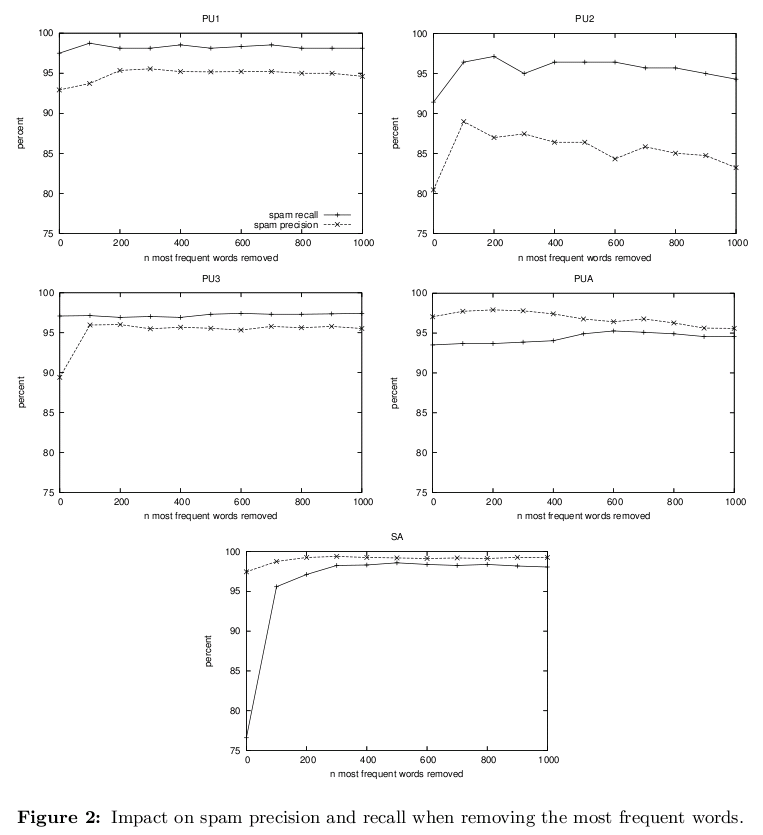
\includegraphics[width=.6\textwidth]{frequent}
  \end{center}
\end{frame}
\note{
  \begin{itemize}
  \fontsize{12}{11}\selectfont
  \item Have a major effect on both precision and recall
  \item Most significant on the largest and non-preprocessed SA corpus where recall increased from 77\% to over 95\% by just removing the hundred most common tokens, but classification gained from removing the 100-200 most frequent tokens on all corpora.
  \item Removing too many tokens reduced classification performance - most notably on the smaller PU2 corpus.
  \end{itemize}
}

\begin{frame}[t]{\centerline{n-grams}}
  \begin{center}
  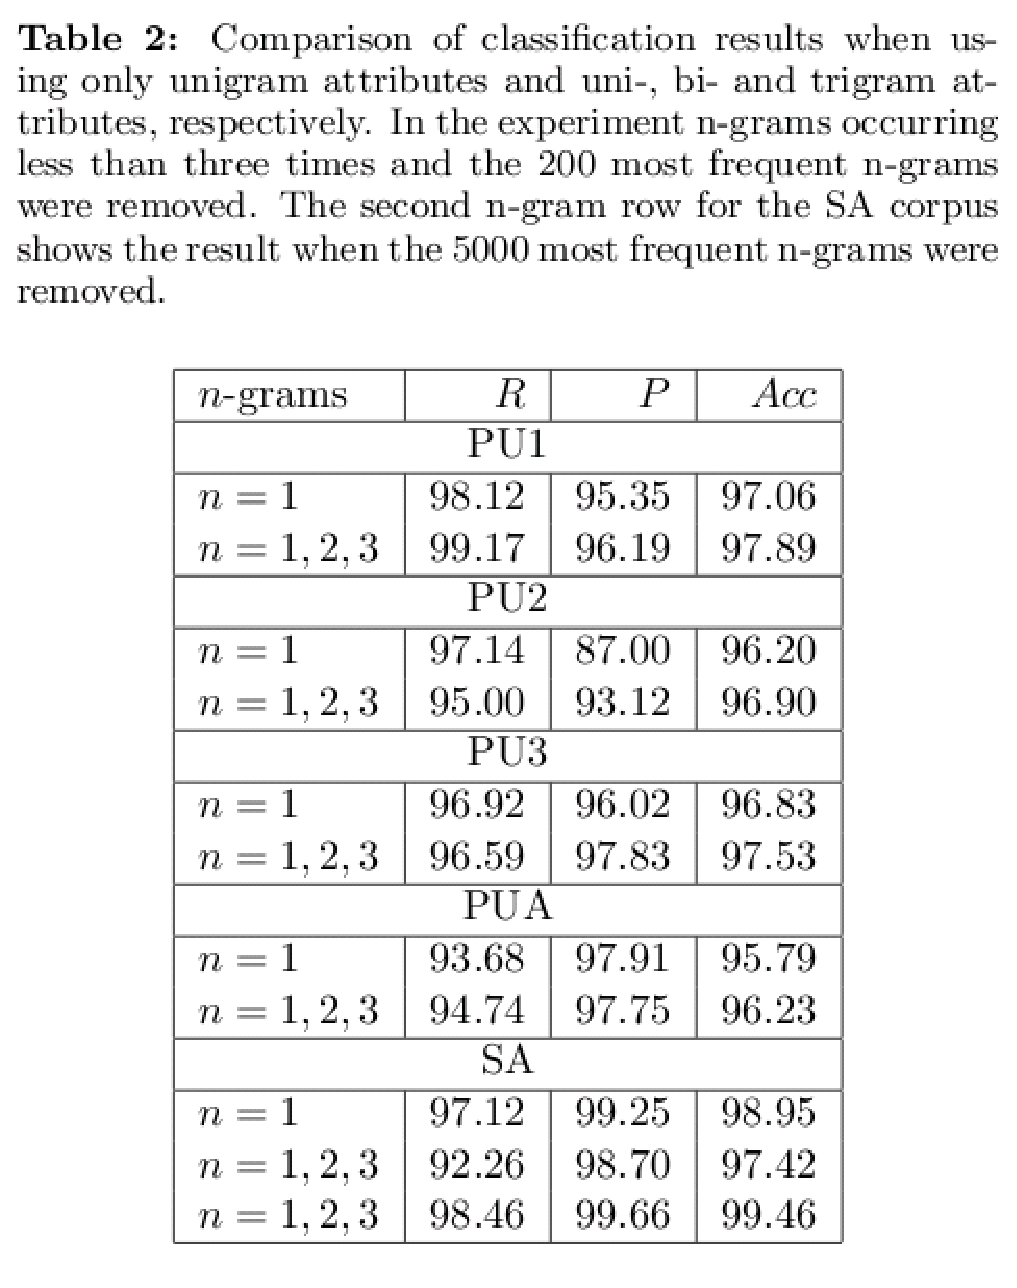
\includegraphics[width=.52\textwidth]{ngram}
  \end{center}
\end{frame}
\note{
  \begin{itemize}
  \item Cost in terms of increased memory requirements 
  \item Consider token sequences of length two and three
  \item Increased classification performance on all of the PU corpora
  \end{itemize}
}

\begin{frame}[t]{\centerline{Cost-Sensitive Classification}}
  \begin{center}
  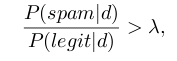
\includegraphics[width=.2\textwidth]{org}
  \end{center}
  \begin{center}
  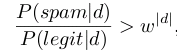
\includegraphics[width=.2\textwidth]{new}
  \end{center}
  \begin{center}
  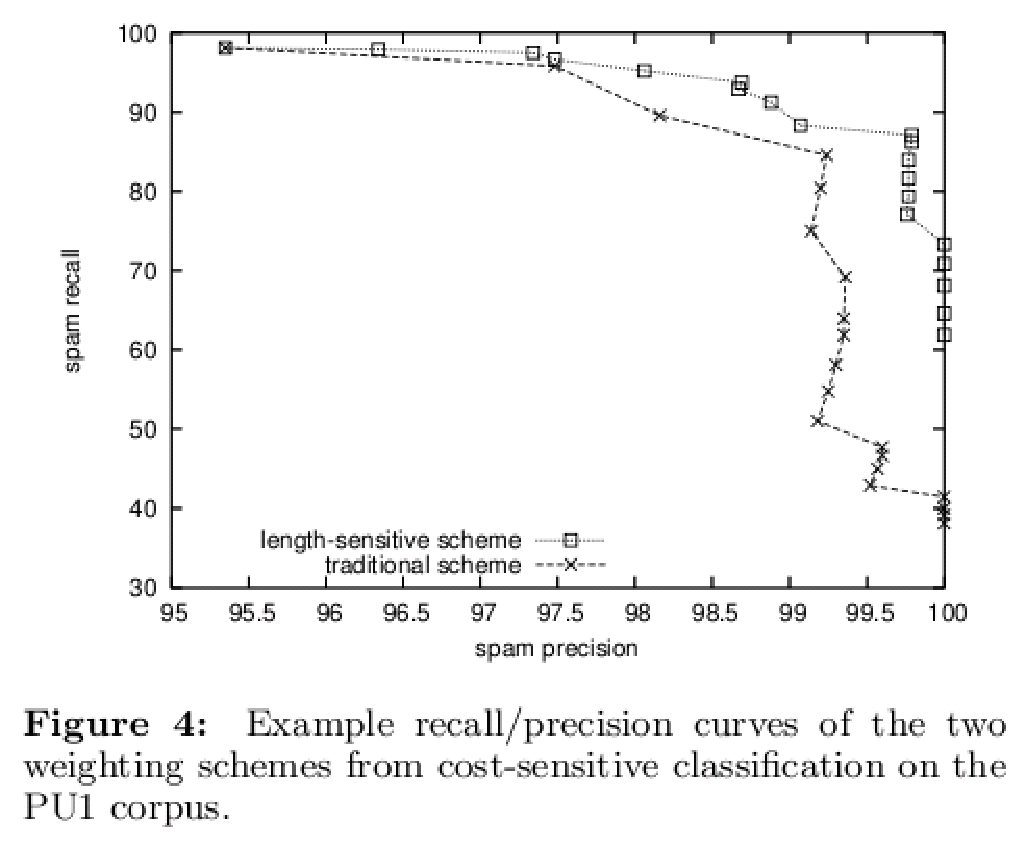
\includegraphics[width=.6\textwidth]{sensitive}
  \end{center}
\end{frame}
\note{
  \begin{itemize}
  \item Bias the filter by make lamda $>$ 1
  \item Naive Bayes classifier is insensitive to (small) changes to lamda since the probability estimates tend to approach 0 and 1, respectively.
  \item This insensitivity increases with the length of the attribute vectors
  \end{itemize}
}

\section{Conclusions}
%\begin{frame}[t]{\centerline{Outline}}
%  \tableofcontents[currentsection]
%\end{frame}
%\note{}

\begin{frame}[t]{\centerline{Conclusion}}
  \ \\
  \begin{itemize}
  \fontsize{13}{11}\selectfont
  \item Possible to achieve very good classification performance using a word-position-based variant of naive Bayes
  \ \\
  \ \\
  \item Attribute selection has been stressed: memory requirements may be lowered and classification performance increased
  \ \\
  \ \\
  \item By extending the attribute set with bi- and trigrams, better classification performance may be achieved
  \ \\
  \ \\
  \item Simple weighting scheme boost precision further
  \end{itemize}
\end{frame}
\note{}

\begin{frame}[t]{\centerline{}}
  \ \\
  \begin{center}
  \begin{Huge}
  \ \\
  \ \\
  Question?
  \end{Huge}
  \end{center}
\end{frame}

\end{document}
